\documentclass[1p]{elsarticle_modified}
%\bibliographystyle{elsarticle-num}

%\usepackage[colorlinks]{hyperref}
%\usepackage{abbrmath_seonhwa} %\Abb, \Ascr, \Acal ,\Abf, \Afrak
\usepackage{amsfonts}
\usepackage{amssymb}
\usepackage{amsmath}
\usepackage{amsthm}
\usepackage{scalefnt}
\usepackage{amsbsy}
\usepackage{kotex}
\usepackage{caption}
\usepackage{subfig}
\usepackage{color}
\usepackage{graphicx}
\usepackage{xcolor} %% white, black, red, green, blue, cyan, magenta, yellow
\usepackage{float}
\usepackage{setspace}
\usepackage{hyperref}

\usepackage{tikz}
\usetikzlibrary{arrows}

\usepackage{multirow}
\usepackage{array} % fixed length table
\usepackage{hhline}

%%%%%%%%%%%%%%%%%%%%%
\makeatletter
\renewcommand*\env@matrix[1][\arraystretch]{%
	\edef\arraystretch{#1}%
	\hskip -\arraycolsep
	\let\@ifnextchar\new@ifnextchar
	\array{*\c@MaxMatrixCols c}}
\makeatother %https://tex.stackexchange.com/questions/14071/how-can-i-increase-the-line-spacing-in-a-matrix
%%%%%%%%%%%%%%%

\usepackage[normalem]{ulem}

\newcommand{\msout}[1]{\ifmmode\text{\sout{\ensuremath{#1}}}\else\sout{#1}\fi}
%SOURCE: \msout is \stkout macro in https://tex.stackexchange.com/questions/20609/strikeout-in-math-mode

\newcommand{\cancel}[1]{
	\ifmmode
	{\color{red}\msout{#1}}
	\else
	{\color{red}\sout{#1}}
	\fi
}

\newcommand{\add}[1]{
	{\color{blue}\uwave{#1}}
}

\newcommand{\replace}[2]{
	\ifmmode
	{\color{red}\msout{#1}}{\color{blue}\uwave{#2}}
	\else
	{\color{red}\sout{#1}}{\color{blue}\uwave{#2}}
	\fi
}

\newcommand{\Sol}{\mathcal{S}} %segment
\newcommand{\D}{D} %diagram
\newcommand{\A}{\mathcal{A}} %arc


%%%%%%%%%%%%%%%%%%%%%%%%%%%%%5 test

\def\sl{\operatorname{\textup{SL}}(2,\Cbb)}
\def\psl{\operatorname{\textup{PSL}}(2,\Cbb)}
\def\quan{\mkern 1mu \triangleright \mkern 1mu}

\theoremstyle{definition}
\newtheorem{thm}{Theorem}[section]
\newtheorem{prop}[thm]{Proposition}
\newtheorem{lem}[thm]{Lemma}
\newtheorem{ques}[thm]{Question}
\newtheorem{cor}[thm]{Corollary}
\newtheorem{defn}[thm]{Definition}
\newtheorem{exam}[thm]{Example}
\newtheorem{rmk}[thm]{Remark}
\newtheorem{alg}[thm]{Algorithm}

\newcommand{\I}{\sqrt{-1}}
\begin{document}

%\begin{frontmatter}
%
%\title{Boundary parabolic representations of knots up to 8 crossings}
%
%%% Group authors per affiliation:
%\author{Yunhi Cho} 
%\address{Department of Mathematics, University of Seoul, Seoul, Korea}
%\ead{yhcho@uos.ac.kr}
%
%
%\author{Seonhwa Kim} %\fnref{s_kim}}
%\address{Center for Geometry and Physics, Institute for Basic Science, Pohang, 37673, Korea}
%\ead{ryeona17@ibs.re.kr}
%
%\author{Hyuk Kim}
%\address{Department of Mathematical Sciences, Seoul National University, Seoul 08826, Korea}
%\ead{hyukkim@snu.ac.kr}
%
%\author{Seokbeom Yoon}
%\address{Department of Mathematical Sciences, Seoul National University, Seoul, 08826,  Korea}
%\ead{sbyoon15@snu.ac.kr}
%
%\begin{abstract}
%We find all boundary parabolic representation of knots up to 8 crossings.
%
%\end{abstract}
%\begin{keyword}
%    \MSC[2010] 57M25 
%\end{keyword}
%
%\end{frontmatter}

%\linenumbers
%\tableofcontents
%
\newcommand\colored[1]{\textcolor{white}{\rule[-0.35ex]{0.8em}{1.4ex}}\kern-0.8em\color{red} #1}%
%\newcommand\colored[1]{\textcolor{white}{ #1}\kern-2.17ex	\textcolor{white}{ #1}\kern-1.81ex	\textcolor{white}{ #1}\kern-2.15ex\color{red}#1	}

{\Large $\underline{12n_{0636}~(K12n_{0636})}$}

\setlength{\tabcolsep}{10pt}
\renewcommand{\arraystretch}{1.6}
\vspace{1cm}\begin{tabular}{m{100pt}>{\centering\arraybackslash}m{274pt}}
\multirow{5}{120pt}{
	\centering
	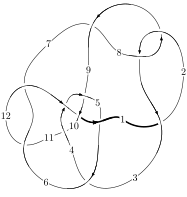
\includegraphics[width=112pt]{../../../GIT/diagram.site/Diagrams/png/2725_12n_0636.png}\\
\ \ \ A knot diagram\footnotemark}&
\allowdisplaybreaks
\textbf{Linearized knot diagam} \\
\cline{2-2}
 &
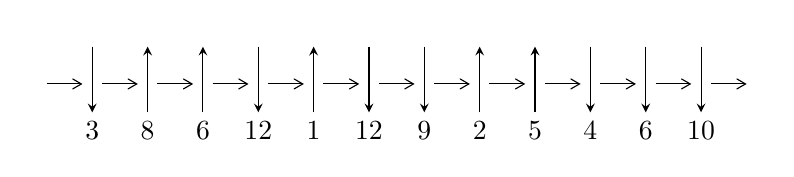
\begin{tikzpicture}[x=20pt, y=17pt]
	% nodes
	\node (C0) at (0, 0) {};
	\node (C1) at (1, 0) {};
	\node (C1U) at (1, +1) {};
	\node (C1D) at (1, -1) {3};

	\node (C2) at (2, 0) {};
	\node (C2U) at (2, +1) {};
	\node (C2D) at (2, -1) {8};

	\node (C3) at (3, 0) {};
	\node (C3U) at (3, +1) {};
	\node (C3D) at (3, -1) {6};

	\node (C4) at (4, 0) {};
	\node (C4U) at (4, +1) {};
	\node (C4D) at (4, -1) {12};

	\node (C5) at (5, 0) {};
	\node (C5U) at (5, +1) {};
	\node (C5D) at (5, -1) {1};

	\node (C6) at (6, 0) {};
	\node (C6U) at (6, +1) {};
	\node (C6D) at (6, -1) {12};

	\node (C7) at (7, 0) {};
	\node (C7U) at (7, +1) {};
	\node (C7D) at (7, -1) {9};

	\node (C8) at (8, 0) {};
	\node (C8U) at (8, +1) {};
	\node (C8D) at (8, -1) {2};

	\node (C9) at (9, 0) {};
	\node (C9U) at (9, +1) {};
	\node (C9D) at (9, -1) {5};

	\node (C10) at (10, 0) {};
	\node (C10U) at (10, +1) {};
	\node (C10D) at (10, -1) {4};

	\node (C11) at (11, 0) {};
	\node (C11U) at (11, +1) {};
	\node (C11D) at (11, -1) {6};

	\node (C12) at (12, 0) {};
	\node (C12U) at (12, +1) {};
	\node (C12D) at (12, -1) {10};
	\node (C13) at (13, 0) {};

	% arrows
	\draw[->,>={angle 60}]
	(C0) edge (C1) (C1) edge (C2) (C2) edge (C3) (C3) edge (C4) (C4) edge (C5) (C5) edge (C6) (C6) edge (C7) (C7) edge (C8) (C8) edge (C9) (C9) edge (C10) (C10) edge (C11) (C11) edge (C12) (C12) edge (C13) ;	\draw[->,>=stealth]
	(C1U) edge (C1D) (C2D) edge (C2U) (C3D) edge (C3U) (C4U) edge (C4D) (C5D) edge (C5U) (C6U) edge (C6D) (C7U) edge (C7D) (C8D) edge (C8U) (C9D) edge (C9U) (C10U) edge (C10D) (C11U) edge (C11D) (C12U) edge (C12D) ;
	\end{tikzpicture} \\
\hhline{~~} \\& 
\textbf{Solving Sequence} \\ \cline{2-2} 
 &
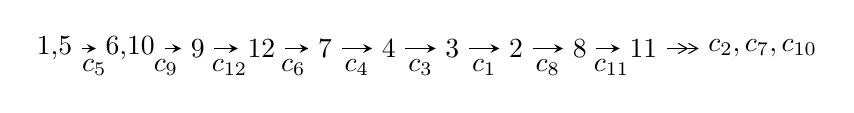
\begin{tikzpicture}[x=23pt, y=7pt]
	% node
	\node (A0) at (-1/8, 0) {1,5};
	\node (A1) at (17/16, 0) {6,10};
	\node (A2) at (17/8, 0) {9};
	\node (A3) at (25/8, 0) {12};
	\node (A4) at (33/8, 0) {7};
	\node (A5) at (41/8, 0) {4};
	\node (A6) at (49/8, 0) {3};
	\node (A7) at (57/8, 0) {2};
	\node (A8) at (65/8, 0) {8};
	\node (A9) at (73/8, 0) {11};
	\node (C1) at (1/2, -1) {$c_{5}$};
	\node (C2) at (13/8, -1) {$c_{9}$};
	\node (C3) at (21/8, -1) {$c_{12}$};
	\node (C4) at (29/8, -1) {$c_{6}$};
	\node (C5) at (37/8, -1) {$c_{4}$};
	\node (C6) at (45/8, -1) {$c_{3}$};
	\node (C7) at (53/8, -1) {$c_{1}$};
	\node (C8) at (61/8, -1) {$c_{8}$};
	\node (C9) at (69/8, -1) {$c_{11}$};
	\node (A10) at (11, 0) {$c_{2},c_{7},c_{10}$};

	% edge
	\draw[->,>=stealth]	
	(A0) edge (A1) (A1) edge (A2) (A2) edge (A3) (A3) edge (A4) (A4) edge (A5) (A5) edge (A6) (A6) edge (A7) (A7) edge (A8) (A8) edge (A9) ;
	\draw[->>,>={angle 60}]	
	(A9) edge (A10);
\end{tikzpicture} \\ 

\end{tabular} \\

\footnotetext{
The image of knot diagram is generated by the software ``\textbf{Draw programme}" developed by Andrew Bartholomew(\url{http://www.layer8.co.uk/maths/draw/index.htm\#Running-draw}), where we modified some parts for our purpose(\url{https://github.com/CATsTAILs/LinksPainter}).
}\phantom \\ \newline 
\centering \textbf{Ideals for irreducible components\footnotemark of $X_{\text{par}}$} 
 
\begin{align*}
I^u_{1}&=\langle 
b- u,\;1.29424\times10^{29} u^{28}-4.50885\times10^{29} u^{27}+\cdots+1.80747\times10^{27} a+2.71900\times10^{29},\\
\phantom{I^u_{1}}&\phantom{= \langle  }u^{29}-4 u^{28}+\cdots+41 u^2-1\rangle \\
I^u_{2}&=\langle 
b+u,\;-1.14135\times10^{17} u^{24}+9.49047\times10^{15} u^{23}+\cdots+2.50582\times10^{16} a+3.47140\times10^{17},\\
\phantom{I^u_{2}}&\phantom{= \langle  }u^{25}+3 u^{23}+\cdots-4 u-1\rangle \\
I^u_{3}&=\langle 
5.05848\times10^{26} u^{23}+1.72101\times10^{27} u^{22}+\cdots+1.51027\times10^{28} b-1.97809\times10^{29},\\
\phantom{I^u_{3}}&\phantom{= \langle  }1.66317\times10^{24} u^{23}+5.60162\times10^{24} u^{22}+\cdots+2.05980\times10^{25} a-6.95407\times10^{26},\\
\phantom{I^u_{3}}&\phantom{= \langle  }u^{24}+3 u^{23}+\cdots-916 u+152\rangle \\
I^u_{4}&=\langle 
b+1,\;3 u^3-8 u^2+4 a+9 u-5,\;u^4-4 u^3+7 u^2-7 u+4\rangle \\
I^u_{5}&=\langle 
b+1,\;a^4-3 a^3+5 a^2-3 a+2,\;u+1\rangle \\
I^u_{6}&=\langle 
- a^3- a^2+b- a-1,\;a^4+a^3+a^2+1,\;u+1\rangle \\
\\
\end{align*}
\raggedright * 6 irreducible components of $\dim_{\mathbb{C}}=0$, with total 90 representations.\\
\footnotetext{All coefficients of polynomials are rational numbers. But the coefficients are sometimes approximated in decimal forms when there is not enough margin.}
\newpage
\renewcommand{\arraystretch}{1}
\centering \section*{I. $I^u_{1}= \langle b- u,\;1.29\times10^{29} u^{28}-4.51\times10^{29} u^{27}+\cdots+1.81\times10^{27} a+2.72\times10^{29},\;u^{29}-4 u^{28}+\cdots+41 u^2-1 \rangle$}
\flushleft \textbf{(i) Arc colorings}\\
\begin{tabular}{m{7pt} m{180pt} m{7pt} m{180pt} }
\flushright $a_{1}=$&$\begin{pmatrix}0\\u\end{pmatrix}$ \\
\flushright $a_{5}=$&$\begin{pmatrix}1\\0\end{pmatrix}$ \\
\flushright $a_{6}=$&$\begin{pmatrix}1\\- u^2\end{pmatrix}$ \\
\flushright $a_{10}=$&$\begin{pmatrix}-71.6051 u^{28}+249.456 u^{27}+\cdots-223.148 u-150.431\\u\end{pmatrix}$ \\
\flushright $a_{9}=$&$\begin{pmatrix}-71.6051 u^{28}+249.456 u^{27}+\cdots-224.148 u-150.431\\u\end{pmatrix}$ \\
\flushright $a_{12}=$&$\begin{pmatrix}-11.9756 u^{28}+39.5117 u^{27}+\cdots+56.9931 u-41.0153\\-18.4538 u^{28}+64.5320 u^{27}+\cdots-70.6051 u-36.9640\end{pmatrix}$ \\
\flushright $a_{7}=$&$\begin{pmatrix}7.86693 u^{28}-25.7993 u^{27}+\cdots-20.9730 u+45.9410\\-19.6452 u^{28}+68.7556 u^{27}+\cdots-79.1491 u-38.6368\end{pmatrix}$ \\
\flushright $a_{4}=$&$\begin{pmatrix}-3.16963 u^{28}+10.4056 u^{27}+\cdots+11.0912 u-19.1412\\20.6054 u^{28}-72.0642 u^{27}+\cdots+82.3187 u+40.9096\end{pmatrix}$ \\
\flushright $a_{3}=$&$\begin{pmatrix}-22.8148 u^{28}+79.1613 u^{27}+\cdots-68.0578 u-57.7779\\25.5368 u^{28}-89.2904 u^{27}+\cdots+101.964 u+50.7349\end{pmatrix}$ \\
\flushright $a_{2}=$&$\begin{pmatrix}28.1973 u^{28}-97.3373 u^{27}+\cdots+82.3877 u+69.1927\\-18.7535 u^{28}+65.8134 u^{27}+\cdots-77.9114 u-37.4792\end{pmatrix}$ \\
\flushright $a_{8}=$&$\begin{pmatrix}-36.1766 u^{28}+127.011 u^{27}+\cdots-157.595 u-62.5413\\-25.5368 u^{28}+89.2904 u^{27}+\cdots-101.964 u-50.7349\end{pmatrix}$ \\
\flushright $a_{11}=$&$\begin{pmatrix}-34.4315 u^{28}+118.013 u^{27}+\cdots-25.5876 u-86.3700\\-12.7801 u^{28}+44.6947 u^{27}+\cdots-48.1492 u-25.6417\end{pmatrix}$\\&\end{tabular}
\flushleft \textbf{(ii) Obstruction class $= -1$}\\~\\
\flushleft \textbf{(iii) Cusp Shapes $= -362.367 u^{28}+1266.86 u^{27}+\cdots-1402.63 u-756.448$}\\~\\
\newpage\renewcommand{\arraystretch}{1}
\flushleft \textbf{(iv) u-Polynomials at the component}\newline \\
\begin{tabular}{m{50pt}|m{274pt}}
Crossings & \hspace{64pt}u-Polynomials at each crossing \\
\hline $$\begin{aligned}c_{1},c_{7}\end{aligned}$$&$\begin{aligned}
&u^{29}+8 u^{28}+\cdots+160 u-64
\end{aligned}$\\
\hline $$\begin{aligned}c_{2},c_{8}\end{aligned}$$&$\begin{aligned}
&u^{29}+8 u^{28}+\cdots+16 u+8
\end{aligned}$\\
\hline $$\begin{aligned}c_{3}\end{aligned}$$&$\begin{aligned}
&u^{29}+15 u^{28}+\cdots+496 u+64
\end{aligned}$\\
\hline $$\begin{aligned}c_{4}\end{aligned}$$&$\begin{aligned}
&u^{29}+2 u^{28}+\cdots+5 u+13
\end{aligned}$\\
\hline $$\begin{aligned}c_{5},c_{9}\end{aligned}$$&$\begin{aligned}
&u^{29}+4 u^{28}+\cdots-41 u^2+1
\end{aligned}$\\
\hline $$\begin{aligned}c_{6},c_{10},c_{11}\end{aligned}$$&$\begin{aligned}
&u^{29}+24 u^{27}+\cdots+5 u+1
\end{aligned}$\\
\hline $$\begin{aligned}c_{12}\end{aligned}$$&$\begin{aligned}
&u^{29}-13 u^{28}+\cdots-100 u+8
\end{aligned}$\\
\hline
\end{tabular}\\~\\
\newpage\renewcommand{\arraystretch}{1}
\flushleft \textbf{(v) Riley Polynomials at the component}\newline \\
\begin{tabular}{m{50pt}|m{274pt}}
Crossings & \hspace{64pt}Riley Polynomials at each crossing \\
\hline $$\begin{aligned}c_{1},c_{7}\end{aligned}$$&$\begin{aligned}
&y^{29}+24 y^{28}+\cdots+94720 y-4096
\end{aligned}$\\
\hline $$\begin{aligned}c_{2},c_{8}\end{aligned}$$&$\begin{aligned}
&y^{29}+8 y^{28}+\cdots+160 y-64
\end{aligned}$\\
\hline $$\begin{aligned}c_{3}\end{aligned}$$&$\begin{aligned}
&y^{29}-35 y^{28}+\cdots+24832 y-4096
\end{aligned}$\\
\hline $$\begin{aligned}c_{4}\end{aligned}$$&$\begin{aligned}
&y^{29}+30 y^{28}+\cdots-1041 y-169
\end{aligned}$\\
\hline $$\begin{aligned}c_{5},c_{9}\end{aligned}$$&$\begin{aligned}
&y^{29}-20 y^{28}+\cdots+82 y-1
\end{aligned}$\\
\hline $$\begin{aligned}c_{6},c_{10},c_{11}\end{aligned}$$&$\begin{aligned}
&y^{29}+48 y^{28}+\cdots-15 y-1
\end{aligned}$\\
\hline $$\begin{aligned}c_{12}\end{aligned}$$&$\begin{aligned}
&y^{29}-3 y^{28}+\cdots-560 y-64
\end{aligned}$\\
\hline
\end{tabular}\\~\\
\newpage\flushleft \textbf{(vi) Complex Volumes and Cusp Shapes}
$$\begin{array}{c|c|c}  
\text{Solutions to }I^u_{1}& \I (\text{vol} + \sqrt{-1}CS) & \text{Cusp shape}\\
 \hline 
\begin{aligned}
u &= \phantom{-}0.960292 + 0.114322 I \\
a &= -0.295102 - 0.789708 I \\
b &= \phantom{-}0.960292 + 0.114322 I\end{aligned}
 & \phantom{-}4.26314 + 5.68742 I & \phantom{-}0.21225 - 6.40052 I \\ \hline\begin{aligned}
u &= \phantom{-}0.960292 - 0.114322 I \\
a &= -0.295102 + 0.789708 I \\
b &= \phantom{-}0.960292 - 0.114322 I\end{aligned}
 & \phantom{-}4.26314 - 5.68742 I & \phantom{-}0.21225 + 6.40052 I \\ \hline\begin{aligned}
u &= -0.800224 + 0.473422 I \\
a &= -0.020933 + 0.683003 I \\
b &= -0.800224 + 0.473422 I\end{aligned}
 & \phantom{-}1.38041 - 0.94269 I & \phantom{-}4.60342 + 1.76965 I \\ \hline\begin{aligned}
u &= -0.800224 - 0.473422 I \\
a &= -0.020933 - 0.683003 I \\
b &= -0.800224 - 0.473422 I\end{aligned}
 & \phantom{-}1.38041 + 0.94269 I & \phantom{-}4.60342 - 1.76965 I \\ \hline\begin{aligned}
u &= \phantom{-}0.214505 + 0.830763 I \\
a &= \phantom{-}0.085940 + 0.697105 I \\
b &= \phantom{-}0.214505 + 0.830763 I\end{aligned}
 & -0.18552 - 2.10133 I & -2.36676 + 3.80844 I \\ \hline\begin{aligned}
u &= \phantom{-}0.214505 - 0.830763 I \\
a &= \phantom{-}0.085940 - 0.697105 I \\
b &= \phantom{-}0.214505 - 0.830763 I\end{aligned}
 & -0.18552 + 2.10133 I & -2.36676 - 3.80844 I \\ \hline\begin{aligned}
u &= \phantom{-}0.834842 + 0.841974 I \\
a &= \phantom{-}0.065712 + 0.604077 I \\
b &= \phantom{-}0.834842 + 0.841974 I\end{aligned}
 & -2.03034 + 3.15669 I & -2.00000 - 3.13089 I \\ \hline\begin{aligned}
u &= \phantom{-}0.834842 - 0.841974 I \\
a &= \phantom{-}0.065712 - 0.604077 I \\
b &= \phantom{-}0.834842 - 0.841974 I\end{aligned}
 & -2.03034 - 3.15669 I & -2.00000 + 3.13089 I \\ \hline\begin{aligned}
u &= -1.170000 + 0.647600 I \\
a &= \phantom{-}0.207159 + 1.203770 I \\
b &= -1.170000 + 0.647600 I\end{aligned}
 & \phantom{-}5.63179 - 9.07757 I & \phantom{-0.000000 } 0 \\ \hline\begin{aligned}
u &= -1.170000 - 0.647600 I \\
a &= \phantom{-}0.207159 - 1.203770 I \\
b &= -1.170000 - 0.647600 I\end{aligned}
 & \phantom{-}5.63179 + 9.07757 I & \phantom{-0.000000 } 0\\
 \hline 
 \end{array}$$\newpage$$\begin{array}{c|c|c}  
\text{Solutions to }I^u_{1}& \I (\text{vol} + \sqrt{-1}CS) & \text{Cusp shape}\\
 \hline 
\begin{aligned}
u &= \phantom{-}1.322730 + 0.290095 I \\
a &= -0.615161 + 1.063240 I \\
b &= \phantom{-}1.322730 + 0.290095 I\end{aligned}
 & \phantom{-}9.61338 + 4.40602 I & \phantom{-0.000000 } 0 \\ \hline\begin{aligned}
u &= \phantom{-}1.322730 - 0.290095 I \\
a &= -0.615161 - 1.063240 I \\
b &= \phantom{-}1.322730 - 0.290095 I\end{aligned}
 & \phantom{-}9.61338 - 4.40602 I & \phantom{-0.000000 } 0 \\ \hline\begin{aligned}
u &= -1.151990 + 0.728821 I \\
a &= \phantom{-}0.002396 + 0.567381 I \\
b &= -1.151990 + 0.728821 I\end{aligned}
 & \phantom{-}4.32796 - 2.63394 I & \phantom{-0.000000 } 0 \\ \hline\begin{aligned}
u &= -1.151990 - 0.728821 I \\
a &= \phantom{-}0.002396 - 0.567381 I \\
b &= -1.151990 - 0.728821 I\end{aligned}
 & \phantom{-}4.32796 + 2.63394 I & \phantom{-0.000000 } 0 \\ \hline\begin{aligned}
u &= -1.171900 + 0.729482 I \\
a &= \phantom{-}1.156260 - 0.116734 I \\
b &= -1.171900 + 0.729482 I\end{aligned}
 & \phantom{-}12.9658 - 7.6542 I & \phantom{-0.000000 } 0 \\ \hline\begin{aligned}
u &= -1.171900 - 0.729482 I \\
a &= \phantom{-}1.156260 + 0.116734 I \\
b &= -1.171900 - 0.729482 I\end{aligned}
 & \phantom{-}12.9658 + 7.6542 I & \phantom{-0.000000 } 0 \\ \hline\begin{aligned}
u &= \phantom{-}1.29794 + 0.56457 I \\
a &= -1.101150 - 0.319489 I \\
b &= \phantom{-}1.29794 + 0.56457 I\end{aligned}
 & \phantom{-}14.08170 + 0.96061 I & \phantom{-0.000000 } 0 \\ \hline\begin{aligned}
u &= \phantom{-}1.29794 - 0.56457 I \\
a &= -1.101150 + 0.319489 I \\
b &= \phantom{-}1.29794 - 0.56457 I\end{aligned}
 & \phantom{-}14.08170 - 0.96061 I & \phantom{-0.000000 } 0 \\ \hline\begin{aligned}
u &= \phantom{-}1.16421 + 0.82395 I \\
a &= \phantom{-}0.013535 + 0.551844 I \\
b &= \phantom{-}1.16421 + 0.82395 I\end{aligned}
 & \phantom{-}3.49095 + 8.40992 I & \phantom{-0.000000 } 0 \\ \hline\begin{aligned}
u &= \phantom{-}1.16421 - 0.82395 I \\
a &= \phantom{-}0.013535 - 0.551844 I \\
b &= \phantom{-}1.16421 - 0.82395 I\end{aligned}
 & \phantom{-}3.49095 - 8.40992 I & \phantom{-0.000000 } 0\\
 \hline 
 \end{array}$$\newpage$$\begin{array}{c|c|c}  
\text{Solutions to }I^u_{1}& \I (\text{vol} + \sqrt{-1}CS) & \text{Cusp shape}\\
 \hline 
\begin{aligned}
u &= \phantom{-}0.498483 + 0.001453 I \\
a &= \phantom{-}0.228167 - 1.207220 I \\
b &= \phantom{-}0.498483 + 0.001453 I\end{aligned}
 & -0.76521 + 1.33560 I & -4.03541 - 5.87673 I \\ \hline\begin{aligned}
u &= \phantom{-}0.498483 - 0.001453 I \\
a &= \phantom{-}0.228167 + 1.207220 I \\
b &= \phantom{-}0.498483 - 0.001453 I\end{aligned}
 & -0.76521 - 1.33560 I & -4.03541 + 5.87673 I \\ \hline\begin{aligned}
u &= \phantom{-}0.233111\phantom{ +0.000000I} \\
a &= \phantom{-}5.33841\phantom{ +0.000000I} \\
b &= \phantom{-}0.233111\phantom{ +0.000000I}\end{aligned}
 & -1.74928\phantom{ +0.000000I} & -9.97660\phantom{ +0.000000I} \\ \hline\begin{aligned}
u &= -0.179695 + 0.046426 I \\
a &= -8.32456 - 5.44841 I \\
b &= -0.179695 + 0.046426 I\end{aligned}
 & -5.01406 - 4.22563 I & -16.2179 - 14.6298 I \\ \hline\begin{aligned}
u &= -0.179695 - 0.046426 I \\
a &= -8.32456 + 5.44841 I \\
b &= -0.179695 - 0.046426 I\end{aligned}
 & -5.01406 + 4.22563 I & -16.2179 + 14.6298 I \\ \hline\begin{aligned}
u &= \phantom{-}1.60072 + 0.97916 I \\
a &= -0.124611 + 0.805147 I \\
b &= \phantom{-}1.60072 + 0.97916 I\end{aligned}
 & \phantom{-}14.8695 + 9.1201 I & \phantom{-0.000000 } 0 \\ \hline\begin{aligned}
u &= \phantom{-}1.60072 - 0.97916 I \\
a &= -0.124611 - 0.805147 I \\
b &= \phantom{-}1.60072 - 0.97916 I\end{aligned}
 & \phantom{-}14.8695 - 9.1201 I & \phantom{-0.000000 } 0 \\ \hline\begin{aligned}
u &= -1.53648 + 1.11077 I \\
a &= \phantom{-}0.053142 + 0.796682 I \\
b &= -1.53648 + 1.11077 I\end{aligned}
 & \phantom{-}13.9120 - 15.6954 I & \phantom{-0.000000 } 0 \\ \hline\begin{aligned}
u &= -1.53648 - 1.11077 I \\
a &= \phantom{-}0.053142 - 0.796682 I \\
b &= -1.53648 - 1.11077 I\end{aligned}
 & \phantom{-}13.9120 + 15.6954 I & \phantom{-0.000000 } 0\\
 \hline 
 \end{array}$$\newpage\newpage\renewcommand{\arraystretch}{1}
\centering \section*{II. $I^u_{2}= \langle b+u,\;-1.14\times10^{17} u^{24}+9.49\times10^{15} u^{23}+\cdots+2.51\times10^{16} a+3.47\times10^{17},\;u^{25}+3 u^{23}+\cdots-4 u-1 \rangle$}
\flushleft \textbf{(i) Arc colorings}\\
\begin{tabular}{m{7pt} m{180pt} m{7pt} m{180pt} }
\flushright $a_{1}=$&$\begin{pmatrix}0\\u\end{pmatrix}$ \\
\flushright $a_{5}=$&$\begin{pmatrix}1\\0\end{pmatrix}$ \\
\flushright $a_{6}=$&$\begin{pmatrix}1\\- u^2\end{pmatrix}$ \\
\flushright $a_{10}=$&$\begin{pmatrix}4.55481 u^{24}-0.378737 u^{23}+\cdots-23.2828 u-13.8534\\- u\end{pmatrix}$ \\
\flushright $a_{9}=$&$\begin{pmatrix}4.55481 u^{24}-0.378737 u^{23}+\cdots-22.2828 u-13.8534\\- u\end{pmatrix}$ \\
\flushright $a_{12}=$&$\begin{pmatrix}11.3465 u^{24}-3.75211 u^{23}+\cdots-53.6177 u-24.6474\\0.463760 u^{24}-0.563270 u^{23}+\cdots-2.03987 u+0.378737\end{pmatrix}$ \\
\flushright $a_{7}=$&$\begin{pmatrix}-13.8534 u^{24}+4.55481 u^{23}+\cdots+73.9510 u+33.1307\\-0.127690 u^{24}-0.228930 u^{23}+\cdots+1.62932 u+0.250675\end{pmatrix}$ \\
\flushright $a_{4}=$&$\begin{pmatrix}-3.62126 u^{24}+1.46376 u^{23}+\cdots+17.6341 u+9.44519\\0.690960 u^{24}-0.0116943 u^{23}+\cdots-3.86310 u-1.71443\end{pmatrix}$ \\
\flushright $a_{3}=$&$\begin{pmatrix}-3.74895 u^{24}+1.23483 u^{23}+\cdots+19.2634 u+9.69586\\0.388246 u^{24}+0.192434 u^{23}+\cdots-2.81969 u-1.48550\end{pmatrix}$ \\
\flushright $a_{2}=$&$\begin{pmatrix}-6.66089 u^{24}+2.95614 u^{23}+\cdots+33.1139 u+11.4051\\0.871238 u^{24}-0.115442 u^{23}+\cdots-3.96879 u-1.75674\end{pmatrix}$ \\
\flushright $a_{8}=$&$\begin{pmatrix}-2.92829 u^{24}+0.509793 u^{23}+\cdots+17.3146 u+9.64795\\-0.388246 u^{24}-0.192434 u^{23}+\cdots+2.81969 u+1.48550\end{pmatrix}$ \\
\flushright $a_{11}=$&$\begin{pmatrix}12.5972 u^{24}-3.87980 u^{23}+\cdots-59.3194 u-28.0208\\0.692691 u^{24}-0.865985 u^{23}+\cdots-2.77978 u+0.506427\end{pmatrix}$\\&\end{tabular}
\flushleft \textbf{(ii) Obstruction class $= 1$}\\~\\
\flushleft \textbf{(iii) Cusp Shapes $= -\frac{141347430048502710}{4176363078274867} u^{24}+\frac{49486291278266828}{4176363078274867} u^{23}+\cdots+\frac{739293424200395475}{4176363078274867} u+\frac{319470269701535049}{4176363078274867}$}\\~\\
\newpage\renewcommand{\arraystretch}{1}
\flushleft \textbf{(iv) u-Polynomials at the component}\newline \\
\begin{tabular}{m{50pt}|m{274pt}}
Crossings & \hspace{64pt}u-Polynomials at each crossing \\
\hline $$\begin{aligned}c_{1},c_{7}\end{aligned}$$&$\begin{aligned}
&u^{25}-10 u^{24}+\cdots-44 u+4
\end{aligned}$\\
\hline $$\begin{aligned}c_{2}\end{aligned}$$&$\begin{aligned}
&u^{25}+5 u^{23}+\cdots+11 u^2+2
\end{aligned}$\\
\hline $$\begin{aligned}c_{3}\end{aligned}$$&$\begin{aligned}
&u^{25}+19 u^{24}+\cdots-21 u+41
\end{aligned}$\\
\hline $$\begin{aligned}c_{4}\end{aligned}$$&$\begin{aligned}
&u^{25}- u^{24}+\cdots-17 u^2+2
\end{aligned}$\\
\hline $$\begin{aligned}c_{5},c_{9}\end{aligned}$$&$\begin{aligned}
&u^{25}+3 u^{23}+\cdots-4 u-1
\end{aligned}$\\
\hline $$\begin{aligned}c_{6},c_{10}\end{aligned}$$&$\begin{aligned}
&u^{25}+7 u^{23}+\cdots- u-1
\end{aligned}$\\
\hline $$\begin{aligned}c_{8}\end{aligned}$$&$\begin{aligned}
&u^{25}+5 u^{23}+\cdots-11 u^2-2
\end{aligned}$\\
\hline $$\begin{aligned}c_{11}\end{aligned}$$&$\begin{aligned}
&u^{25}+7 u^{23}+\cdots- u+1
\end{aligned}$\\
\hline $$\begin{aligned}c_{12}\end{aligned}$$&$\begin{aligned}
&u^{25}+11 u^{24}+\cdots-7 u^2+1
\end{aligned}$\\
\hline
\end{tabular}\\~\\
\newpage\renewcommand{\arraystretch}{1}
\flushleft \textbf{(v) Riley Polynomials at the component}\newline \\
\begin{tabular}{m{50pt}|m{274pt}}
Crossings & \hspace{64pt}Riley Polynomials at each crossing \\
\hline $$\begin{aligned}c_{1},c_{7}\end{aligned}$$&$\begin{aligned}
&y^{25}+18 y^{24}+\cdots-24 y-16
\end{aligned}$\\
\hline $$\begin{aligned}c_{2},c_{8}\end{aligned}$$&$\begin{aligned}
&y^{25}+10 y^{24}+\cdots-44 y-4
\end{aligned}$\\
\hline $$\begin{aligned}c_{3}\end{aligned}$$&$\begin{aligned}
&y^{25}-35 y^{24}+\cdots+70715 y-1681
\end{aligned}$\\
\hline $$\begin{aligned}c_{4}\end{aligned}$$&$\begin{aligned}
&y^{25}+11 y^{24}+\cdots+68 y-4
\end{aligned}$\\
\hline $$\begin{aligned}c_{5},c_{9}\end{aligned}$$&$\begin{aligned}
&y^{25}+6 y^{24}+\cdots+10 y-1
\end{aligned}$\\
\hline $$\begin{aligned}c_{6},c_{10},c_{11}\end{aligned}$$&$\begin{aligned}
&y^{25}+14 y^{24}+\cdots+17 y-1
\end{aligned}$\\
\hline $$\begin{aligned}c_{12}\end{aligned}$$&$\begin{aligned}
&y^{25}-3 y^{24}+\cdots+14 y-1
\end{aligned}$\\
\hline
\end{tabular}\\~\\
\newpage\flushleft \textbf{(vi) Complex Volumes and Cusp Shapes}
$$\begin{array}{c|c|c}  
\text{Solutions to }I^u_{2}& \I (\text{vol} + \sqrt{-1}CS) & \text{Cusp shape}\\
 \hline 
\begin{aligned}
u &= \phantom{-}0.796080 + 0.645844 I \\
a &= -0.596796 - 0.240010 I \\
b &= -0.796080 - 0.645844 I\end{aligned}
 & \phantom{-}4.84322 - 2.05050 I & \phantom{-}0.28599 - 1.48631 I \\ \hline\begin{aligned}
u &= \phantom{-}0.796080 - 0.645844 I \\
a &= -0.596796 + 0.240010 I \\
b &= -0.796080 + 0.645844 I\end{aligned}
 & \phantom{-}4.84322 + 2.05050 I & \phantom{-}0.28599 + 1.48631 I \\ \hline\begin{aligned}
u &= \phantom{-}0.296077 + 0.914388 I \\
a &= -0.699710 - 1.211640 I \\
b &= -0.296077 - 0.914388 I\end{aligned}
 & -2.56141 + 2.33620 I & -10.59682 - 7.19824 I \\ \hline\begin{aligned}
u &= \phantom{-}0.296077 - 0.914388 I \\
a &= -0.699710 + 1.211640 I \\
b &= -0.296077 + 0.914388 I\end{aligned}
 & -2.56141 - 2.33620 I & -10.59682 + 7.19824 I \\ \hline\begin{aligned}
u &= \phantom{-}0.922082 + 0.228189 I \\
a &= -0.381519 - 0.872909 I \\
b &= -0.922082 - 0.228189 I\end{aligned}
 & \phantom{-}6.61274 - 0.16294 I & \phantom{-}8.10933 + 0.42456 I \\ \hline\begin{aligned}
u &= \phantom{-}0.922082 - 0.228189 I \\
a &= -0.381519 + 0.872909 I \\
b &= -0.922082 + 0.228189 I\end{aligned}
 & \phantom{-}6.61274 + 0.16294 I & \phantom{-}8.10933 - 0.42456 I \\ \hline\begin{aligned}
u &= -0.809953 + 0.096839 I \\
a &= \phantom{-}0.363322 - 1.250440 I \\
b &= \phantom{-}0.809953 - 0.096839 I\end{aligned}
 & \phantom{-}5.86968 + 5.30210 I & \phantom{-}5.18661 - 5.91989 I \\ \hline\begin{aligned}
u &= -0.809953 - 0.096839 I \\
a &= \phantom{-}0.363322 + 1.250440 I \\
b &= \phantom{-}0.809953 + 0.096839 I\end{aligned}
 & \phantom{-}5.86968 - 5.30210 I & \phantom{-}5.18661 + 5.91989 I \\ \hline\begin{aligned}
u &= -0.687921 + 1.038030 I \\
a &= \phantom{-}0.174351 - 0.908552 I \\
b &= \phantom{-}0.687921 - 1.038030 I\end{aligned}
 & -3.20695 - 4.09541 I & -9.54085 + 4.81505 I \\ \hline\begin{aligned}
u &= -0.687921 - 1.038030 I \\
a &= \phantom{-}0.174351 + 0.908552 I \\
b &= \phantom{-}0.687921 + 1.038030 I\end{aligned}
 & -3.20695 + 4.09541 I & -9.54085 - 4.81505 I\\
 \hline 
 \end{array}$$\newpage$$\begin{array}{c|c|c}  
\text{Solutions to }I^u_{2}& \I (\text{vol} + \sqrt{-1}CS) & \text{Cusp shape}\\
 \hline 
\begin{aligned}
u &= \phantom{-}1.115530 + 0.661232 I \\
a &= \phantom{-}0.315105 - 0.652823 I \\
b &= -1.115530 - 0.661232 I\end{aligned}
 & \phantom{-}3.30766 + 2.48097 I & -1.93779 - 1.88948 I \\ \hline\begin{aligned}
u &= \phantom{-}1.115530 - 0.661232 I \\
a &= \phantom{-}0.315105 + 0.652823 I \\
b &= -1.115530 + 0.661232 I\end{aligned}
 & \phantom{-}3.30766 - 2.48097 I & -1.93779 + 1.88948 I \\ \hline\begin{aligned}
u &= \phantom{-}0.343736 + 1.273220 I \\
a &= -0.539488 - 0.735855 I \\
b &= -0.343736 - 1.273220 I\end{aligned}
 & -0.22260 + 5.42341 I & \phantom{-}0.75618 - 6.73991 I \\ \hline\begin{aligned}
u &= \phantom{-}0.343736 - 1.273220 I \\
a &= -0.539488 + 0.735855 I \\
b &= -0.343736 + 1.273220 I\end{aligned}
 & -0.22260 - 5.42341 I & \phantom{-}0.75618 + 6.73991 I \\ \hline\begin{aligned}
u &= \phantom{-}0.675230\phantom{ +0.000000I} \\
a &= \phantom{-}2.07673\phantom{ +0.000000I} \\
b &= -0.675230\phantom{ +0.000000I}\end{aligned}
 & -1.26232\phantom{ +0.000000I} & \phantom{-}7.41310\phantom{ +0.000000I} \\ \hline\begin{aligned}
u &= -1.125130 + 0.793831 I \\
a &= -0.199464 - 0.663668 I \\
b &= \phantom{-}1.125130 - 0.793831 I\end{aligned}
 & \phantom{-}2.60794 - 8.42230 I & -4.02327 + 7.25592 I \\ \hline\begin{aligned}
u &= -1.125130 - 0.793831 I \\
a &= -0.199464 + 0.663668 I \\
b &= \phantom{-}1.125130 + 0.793831 I\end{aligned}
 & \phantom{-}2.60794 + 8.42230 I & -4.02327 - 7.25592 I \\ \hline\begin{aligned}
u &= -0.454409 + 1.305940 I \\
a &= \phantom{-}0.440942 - 0.724830 I \\
b &= \phantom{-}0.454409 - 1.305940 I\end{aligned}
 & -0.334771 - 0.254683 I & \phantom{-}0.594711 - 0.383137 I \\ \hline\begin{aligned}
u &= -0.454409 - 1.305940 I \\
a &= \phantom{-}0.440942 + 0.724830 I \\
b &= \phantom{-}0.454409 + 1.305940 I\end{aligned}
 & -0.334771 + 0.254683 I & \phantom{-}0.594711 + 0.383137 I \\ \hline\begin{aligned}
u &= -0.440390 + 0.366580 I \\
a &= \phantom{-}1.96302 - 0.28081 I \\
b &= \phantom{-}0.440390 - 0.366580 I\end{aligned}
 & \phantom{-}3.32428 - 0.29299 I & -4.35678 + 0.94699 I\\
 \hline 
 \end{array}$$\newpage$$\begin{array}{c|c|c}  
\text{Solutions to }I^u_{2}& \I (\text{vol} + \sqrt{-1}CS) & \text{Cusp shape}\\
 \hline 
\begin{aligned}
u &= -0.440390 - 0.366580 I \\
a &= \phantom{-}1.96302 + 0.28081 I \\
b &= \phantom{-}0.440390 + 0.366580 I\end{aligned}
 & \phantom{-}3.32428 + 0.29299 I & -4.35678 - 0.94699 I \\ \hline\begin{aligned}
u &= \phantom{-}0.11956 + 1.47573 I \\
a &= -0.042858 + 0.212628 I \\
b &= -0.11956 - 1.47573 I\end{aligned}
 & \phantom{-}11.63180 - 3.18462 I & \phantom{-}3.10708 + 2.38160 I \\ \hline\begin{aligned}
u &= \phantom{-}0.11956 - 1.47573 I \\
a &= -0.042858 - 0.212628 I \\
b &= -0.11956 + 1.47573 I\end{aligned}
 & \phantom{-}11.63180 + 3.18462 I & \phantom{-}3.10708 - 2.38160 I \\ \hline\begin{aligned}
u &= -0.412870 + 0.210392 I \\
a &= -2.83528 - 2.84508 I \\
b &= \phantom{-}0.412870 - 0.210392 I\end{aligned}
 & -4.92153 - 4.38703 I & \phantom{-}5.2090 + 22.1333 I \\ \hline\begin{aligned}
u &= -0.412870 - 0.210392 I \\
a &= -2.83528 + 2.84508 I \\
b &= \phantom{-}0.412870 + 0.210392 I\end{aligned}
 & -4.92153 + 4.38703 I & \phantom{-}5.2090 - 22.1333 I\\
 \hline 
 \end{array}$$\newpage\newpage\renewcommand{\arraystretch}{1}
\centering \section*{III. $I^u_{3}= \langle 5.06\times10^{26} u^{23}+1.72\times10^{27} u^{22}+\cdots+1.51\times10^{28} b-1.98\times10^{29},\;1.66\times10^{24} u^{23}+5.60\times10^{24} u^{22}+\cdots+2.06\times10^{25} a-6.95\times10^{26},\;u^{24}+3 u^{23}+\cdots-916 u+152 \rangle$}
\flushleft \textbf{(i) Arc colorings}\\
\begin{tabular}{m{7pt} m{180pt} m{7pt} m{180pt} }
\flushright $a_{1}=$&$\begin{pmatrix}0\\u\end{pmatrix}$ \\
\flushright $a_{5}=$&$\begin{pmatrix}1\\0\end{pmatrix}$ \\
\flushright $a_{6}=$&$\begin{pmatrix}1\\- u^2\end{pmatrix}$ \\
\flushright $a_{10}=$&$\begin{pmatrix}-0.0807441 u^{23}-0.271949 u^{22}+\cdots-112.103 u+33.7608\\-0.0334939 u^{23}-0.113953 u^{22}+\cdots-45.6844 u+13.0976\end{pmatrix}$ \\
\flushright $a_{9}=$&$\begin{pmatrix}-0.0472503 u^{23}-0.157996 u^{22}+\cdots-66.4189 u+20.6632\\-0.0334939 u^{23}-0.113953 u^{22}+\cdots-45.6844 u+13.0976\end{pmatrix}$ \\
\flushright $a_{12}=$&$\begin{pmatrix}0.0635809 u^{23}+0.212954 u^{22}+\cdots+87.2711 u-27.6880\\0.0521176 u^{23}+0.175261 u^{22}+\cdots+72.2476 u-22.1390\end{pmatrix}$ \\
\flushright $a_{7}=$&$\begin{pmatrix}-0.0561598 u^{23}-0.189820 u^{22}+\cdots-76.9321 u+22.8112\\0.0172861 u^{23}+0.0557112 u^{22}+\cdots+25.6034 u-9.48966\end{pmatrix}$ \\
\flushright $a_{4}=$&$\begin{pmatrix}0.0388737 u^{23}+0.134109 u^{22}+\cdots+51.3287 u-13.3215\\-0.0250608 u^{23}-0.0822551 u^{22}+\cdots-35.7136 u+12.1478\end{pmatrix}$ \\
\flushright $a_{3}=$&$\begin{pmatrix}0.0561598 u^{23}+0.189820 u^{22}+\cdots+76.9321 u-22.8112\\-0.0254832 u^{23}-0.0841583 u^{22}+\cdots-36.6152 u+12.7335\end{pmatrix}$ \\
\flushright $a_{2}=$&$\begin{pmatrix}-0.0472503 u^{23}-0.157996 u^{22}+\cdots-66.4189 u+20.6632\\-0.0278389 u^{23}-0.0949127 u^{22}+\cdots-35.9862 u+10.6284\end{pmatrix}$ \\
\flushright $a_{8}=$&$\begin{pmatrix}-0.0719550 u^{23}-0.242039 u^{22}+\cdots-98.3636 u+29.8284\\-0.0227300 u^{23}-0.0785800 u^{22}+\cdots-30.8874 u+7.99453\end{pmatrix}$ \\
\flushright $a_{11}=$&$\begin{pmatrix}0.123958 u^{23}+0.415686 u^{22}+\cdots+170.200 u-53.2032\\0.0437678 u^{23}+0.146509 u^{22}+\cdots+61.6377 u-18.8555\end{pmatrix}$\\&\end{tabular}
\flushleft \textbf{(ii) Obstruction class $= -1$}\\~\\
\flushleft \textbf{(iii) Cusp Shapes $= \frac{789409549397297077238438255}{1887837650177179023809147344} u^{23}+\frac{5345499614610035395715935423}{3775675300354358047618294688} u^{22}+\cdots+\frac{534181212237586784175387060335}{943918825088589511904573672} u-\frac{81677490050712823192860035961}{471959412544294755952286836}$}\\~\\
\newpage\renewcommand{\arraystretch}{1}
\flushleft \textbf{(iv) u-Polynomials at the component}\newline \\
\begin{tabular}{m{50pt}|m{274pt}}
Crossings & \hspace{64pt}u-Polynomials at each crossing \\
\hline $$\begin{aligned}c_{1},c_{7}\end{aligned}$$&$\begin{aligned}
&(u^4+u^3+3 u^2+2 u+1)^6
\end{aligned}$\\
\hline $$\begin{aligned}c_{2},c_{8}\end{aligned}$$&$\begin{aligned}
&(u^4- u^3+u^2+1)^6
\end{aligned}$\\
\hline $$\begin{aligned}c_{3}\end{aligned}$$&$\begin{aligned}
&(u^4-3 u^3+u^2+2 u+1)^6
\end{aligned}$\\
\hline $$\begin{aligned}c_{4}\end{aligned}$$&$\begin{aligned}
&u^{24}-5 u^{23}+\cdots-19608 u+4792
\end{aligned}$\\
\hline $$\begin{aligned}c_{5},c_{9}\end{aligned}$$&$\begin{aligned}
&u^{24}-3 u^{23}+\cdots+916 u+152
\end{aligned}$\\
\hline $$\begin{aligned}c_{6},c_{10},c_{11}\end{aligned}$$&$\begin{aligned}
&u^{24}-6 u^{23}+\cdots-2820 u+421
\end{aligned}$\\
\hline $$\begin{aligned}c_{12}\end{aligned}$$&$\begin{aligned}
&(u^4+u^3+u^2+1)^6
\end{aligned}$\\
\hline
\end{tabular}\\~\\
\newpage\renewcommand{\arraystretch}{1}
\flushleft \textbf{(v) Riley Polynomials at the component}\newline \\
\begin{tabular}{m{50pt}|m{274pt}}
Crossings & \hspace{64pt}Riley Polynomials at each crossing \\
\hline $$\begin{aligned}c_{1},c_{7}\end{aligned}$$&$\begin{aligned}
&(y^4+5 y^3+7 y^2+2 y+1)^6
\end{aligned}$\\
\hline $$\begin{aligned}c_{2},c_{8},c_{12}\end{aligned}$$&$\begin{aligned}
&(y^4+y^3+3 y^2+2 y+1)^6
\end{aligned}$\\
\hline $$\begin{aligned}c_{3}\end{aligned}$$&$\begin{aligned}
&(y^4-7 y^3+15 y^2-2 y+1)^6
\end{aligned}$\\
\hline $$\begin{aligned}c_{4}\end{aligned}$$&$\begin{aligned}
&y^{24}+13 y^{23}+\cdots+10329632 y+22963264
\end{aligned}$\\
\hline $$\begin{aligned}c_{5},c_{9}\end{aligned}$$&$\begin{aligned}
&y^{24}+9 y^{23}+\cdots-295504 y+23104
\end{aligned}$\\
\hline $$\begin{aligned}c_{6},c_{10},c_{11}\end{aligned}$$&$\begin{aligned}
&y^{24}+34 y^{23}+\cdots-101592 y+177241
\end{aligned}$\\
\hline
\end{tabular}\\~\\
\newpage\flushleft \textbf{(vi) Complex Volumes and Cusp Shapes}
$$\begin{array}{c|c|c}  
\text{Solutions to }I^u_{3}& \I (\text{vol} + \sqrt{-1}CS) & \text{Cusp shape}\\
 \hline 
\begin{aligned}
u &= \phantom{-}0.451653 + 0.937171 I \\
a &= -0.433636 - 1.117900 I \\
b &= -0.128858 - 0.863491 I\end{aligned}
 & -2.06694 + 1.74886 I & -1.65348 + 2.34394 I \\ \hline\begin{aligned}
u &= \phantom{-}0.451653 - 0.937171 I \\
a &= -0.433636 + 1.117900 I \\
b &= -0.128858 + 0.863491 I\end{aligned}
 & -2.06694 - 1.74886 I & -1.65348 - 2.34394 I \\ \hline\begin{aligned}
u &= \phantom{-}0.727252 + 0.755470 I \\
a &= \phantom{-}0.262219 + 0.718105 I \\
b &= -1.54826 + 2.15106 I\end{aligned}
 & \phantom{-}11.93650 + 4.57907 I & \phantom{-}5.65348 - 7.47354 I \\ \hline\begin{aligned}
u &= \phantom{-}0.727252 - 0.755470 I \\
a &= \phantom{-}0.262219 - 0.718105 I \\
b &= -1.54826 - 2.15106 I\end{aligned}
 & \phantom{-}11.93650 - 4.57907 I & \phantom{-}5.65348 + 7.47354 I \\ \hline\begin{aligned}
u &= \phantom{-}0.607909 + 0.908003 I \\
a &= -0.259320 - 1.111730 I \\
b &= -0.615212 - 1.239020 I\end{aligned}
 & -2.06694 + 4.57907 I & -1.65348 - 7.47354 I \\ \hline\begin{aligned}
u &= \phantom{-}0.607909 - 0.908003 I \\
a &= -0.259320 + 1.111730 I \\
b &= -0.615212 + 1.239020 I\end{aligned}
 & -2.06694 - 4.57907 I & -1.65348 + 7.47354 I \\ \hline\begin{aligned}
u &= \phantom{-}1.097460 + 0.195307 I \\
a &= \phantom{-}0.609099 - 0.938762 I \\
b &= -1.56114 - 0.84926 I\end{aligned}
 & \phantom{-}4.93480 + 6.32793 I & \phantom{-}2.00000 - 5.12960 I \\ \hline\begin{aligned}
u &= \phantom{-}1.097460 - 0.195307 I \\
a &= \phantom{-}0.609099 + 0.938762 I \\
b &= -1.56114 + 0.84926 I\end{aligned}
 & \phantom{-}4.93480 - 6.32793 I & \phantom{-}2.00000 + 5.12960 I \\ \hline\begin{aligned}
u &= -0.867738 + 0.717770 I \\
a &= -0.166984 + 0.692013 I \\
b &= \phantom{-}1.29037 + 2.27278 I\end{aligned}
 & \phantom{-}11.93650 + 1.74886 I & \phantom{-}5.65348 + 2.34394 I \\ \hline\begin{aligned}
u &= -0.867738 - 0.717770 I \\
a &= -0.166984 - 0.692013 I \\
b &= \phantom{-}1.29037 - 2.27278 I\end{aligned}
 & \phantom{-}11.93650 - 1.74886 I & \phantom{-}5.65348 - 2.34394 I\\
 \hline 
 \end{array}$$\newpage$$\begin{array}{c|c|c}  
\text{Solutions to }I^u_{3}& \I (\text{vol} + \sqrt{-1}CS) & \text{Cusp shape}\\
 \hline 
\begin{aligned}
u &= -0.128858 + 0.863491 I \\
a &= \phantom{-}0.88836 - 1.11904 I \\
b &= \phantom{-}0.451653 - 0.937171 I\end{aligned}
 & -2.06694 - 1.74886 I & -1.65348 - 2.34394 I \\ \hline\begin{aligned}
u &= -0.128858 - 0.863491 I \\
a &= \phantom{-}0.88836 + 1.11904 I \\
b &= \phantom{-}0.451653 + 0.937171 I\end{aligned}
 & -2.06694 + 1.74886 I & -1.65348 + 2.34394 I \\ \hline\begin{aligned}
u &= -0.615212 + 1.239020 I \\
a &= \phantom{-}0.316184 - 0.844481 I \\
b &= \phantom{-}0.607909 - 0.908003 I\end{aligned}
 & -2.06694 - 4.57907 I & -1.65348 + 7.47354 I \\ \hline\begin{aligned}
u &= -0.615212 - 1.239020 I \\
a &= \phantom{-}0.316184 + 0.844481 I \\
b &= \phantom{-}0.607909 + 0.908003 I\end{aligned}
 & -2.06694 + 4.57907 I & -1.65348 - 7.47354 I \\ \hline\begin{aligned}
u &= -1.31086 + 0.82372 I \\
a &= \phantom{-}0.439962 - 0.273053 I \\
b &= \phantom{-}0.357423 - 0.019370 I\end{aligned}
 & \phantom{-}4.93480 + 2.83021 I & \phantom{-}2.00000 - 9.81749 I \\ \hline\begin{aligned}
u &= -1.31086 - 0.82372 I \\
a &= \phantom{-}0.439962 + 0.273053 I \\
b &= \phantom{-}0.357423 + 0.019370 I\end{aligned}
 & \phantom{-}4.93480 - 2.83021 I & \phantom{-}2.00000 + 9.81749 I \\ \hline\begin{aligned}
u &= \phantom{-}0.357423 + 0.019370 I \\
a &= -1.09031 - 1.95629 I \\
b &= -1.31086 - 0.82372 I\end{aligned}
 & \phantom{-}4.93480 - 2.83021 I & \phantom{-}2.00000 + 9.81749 I \\ \hline\begin{aligned}
u &= \phantom{-}0.357423 - 0.019370 I \\
a &= -1.09031 + 1.95629 I \\
b &= -1.31086 + 0.82372 I\end{aligned}
 & \phantom{-}4.93480 + 2.83021 I & \phantom{-}2.00000 - 9.81749 I \\ \hline\begin{aligned}
u &= -1.56114 + 0.84926 I \\
a &= -0.175996 - 0.679476 I \\
b &= \phantom{-}1.097460 - 0.195307 I\end{aligned}
 & \phantom{-}4.93480 - 6.32793 I & \phantom{-}2.00000 + 5.12960 I \\ \hline\begin{aligned}
u &= -1.56114 - 0.84926 I \\
a &= -0.175996 + 0.679476 I \\
b &= \phantom{-}1.097460 + 0.195307 I\end{aligned}
 & \phantom{-}4.93480 + 6.32793 I & \phantom{-}2.00000 - 5.12960 I\\
 \hline 
 \end{array}$$\newpage$$\begin{array}{c|c|c}  
\text{Solutions to }I^u_{3}& \I (\text{vol} + \sqrt{-1}CS) & \text{Cusp shape}\\
 \hline 
\begin{aligned}
u &= \phantom{-}1.29037 + 2.27278 I \\
a &= -0.306144 - 0.019022 I \\
b &= -0.867738 + 0.717770 I\end{aligned}
 & \phantom{-}11.93650 + 1.74886 I & \phantom{-0.000000 } 0 \\ \hline\begin{aligned}
u &= \phantom{-}1.29037 - 2.27278 I \\
a &= -0.306144 + 0.019022 I \\
b &= -0.867738 - 0.717770 I\end{aligned}
 & \phantom{-}11.93650 - 1.74886 I & \phantom{-0.000000 } 0 \\ \hline\begin{aligned}
u &= -1.54826 + 2.15106 I \\
a &= \phantom{-}0.298140 - 0.051040 I \\
b &= \phantom{-}0.727252 + 0.755470 I\end{aligned}
 & \phantom{-}11.93650 + 4.57907 I & \phantom{-0.000000 } 0 \\ \hline\begin{aligned}
u &= -1.54826 - 2.15106 I \\
a &= \phantom{-}0.298140 + 0.051040 I \\
b &= \phantom{-}0.727252 - 0.755470 I\end{aligned}
 & \phantom{-}11.93650 - 4.57907 I & \phantom{-0.000000 } 0\\
 \hline 
 \end{array}$$\newpage\newpage\renewcommand{\arraystretch}{1}
\centering \section*{IV. $I^u_{4}= \langle b+1,\;3 u^3-8 u^2+4 a+9 u-5,\;u^4-4 u^3+7 u^2-7 u+4 \rangle$}
\flushleft \textbf{(i) Arc colorings}\\
\begin{tabular}{m{7pt} m{180pt} m{7pt} m{180pt} }
\flushright $a_{1}=$&$\begin{pmatrix}0\\u\end{pmatrix}$ \\
\flushright $a_{5}=$&$\begin{pmatrix}1\\0\end{pmatrix}$ \\
\flushright $a_{6}=$&$\begin{pmatrix}1\\- u^2\end{pmatrix}$ \\
\flushright $a_{10}=$&$\begin{pmatrix}-\frac{3}{4} u^3+2 u^2-\frac{9}{4} u+\frac{5}{4}\\-1\end{pmatrix}$ \\
\flushright $a_{9}=$&$\begin{pmatrix}-\frac{3}{4} u^3+2 u^2-\frac{9}{4} u+\frac{9}{4}\\-1\end{pmatrix}$ \\
\flushright $a_{12}=$&$\begin{pmatrix}-\frac{1}{4} u^3+\frac{1}{4} u-\frac{1}{4}\\u^3-3 u^2+5 u-3\end{pmatrix}$ \\
\flushright $a_{7}=$&$\begin{pmatrix}-\frac{1}{4} u^3+\frac{1}{4} u-\frac{1}{4}\\- u^3+3 u^2-3 u+1\end{pmatrix}$ \\
\flushright $a_{4}=$&$\begin{pmatrix}\frac{5}{4} u^3-3 u^2+\frac{11}{4} u-\frac{3}{4}\\- u^3+3 u^2-6 u+7\end{pmatrix}$ \\
\flushright $a_{3}=$&$\begin{pmatrix}\frac{1}{4} u^3-\frac{1}{4} u+\frac{1}{4}\\- u^3+2 u^2-3 u+3\end{pmatrix}$ \\
\flushright $a_{2}=$&$\begin{pmatrix}-\frac{3}{4} u^3+2 u^2-\frac{9}{4} u+\frac{9}{4}\\u^3-4 u^2+6 u-5\end{pmatrix}$ \\
\flushright $a_{8}=$&$\begin{pmatrix}\frac{1}{2} u^3- u^2+\frac{3}{2} u-\frac{1}{2}\\-2 u^3+5 u^2-5 u+2\end{pmatrix}$ \\
\flushright $a_{11}=$&$\begin{pmatrix}-\frac{5}{4} u^3+2 u^2-\frac{3}{4} u+\frac{3}{4}\\3 u^3-11 u^2+15 u-11\end{pmatrix}$\\&\end{tabular}
\flushleft \textbf{(ii) Obstruction class $= -1$}\\~\\
\flushleft \textbf{(iii) Cusp Shapes $= 2$}\\~\\
\newpage\renewcommand{\arraystretch}{1}
\flushleft \textbf{(iv) u-Polynomials at the component}\newline \\
\begin{tabular}{m{50pt}|m{274pt}}
Crossings & \hspace{64pt}u-Polynomials at each crossing \\
\hline $$\begin{aligned}c_{1},c_{7}\end{aligned}$$&$\begin{aligned}
&u^4+u^3+3 u^2+2 u+1
\end{aligned}$\\
\hline $$\begin{aligned}c_{2},c_{8}\end{aligned}$$&$\begin{aligned}
&u^4- u^3+u^2+1
\end{aligned}$\\
\hline $$\begin{aligned}c_{3}\end{aligned}$$&$\begin{aligned}
&u^4-3 u^3+u^2+2 u+1
\end{aligned}$\\
\hline $$\begin{aligned}c_{4}\end{aligned}$$&$\begin{aligned}
&u^4+3 u^3+9 u^2+10 u+11
\end{aligned}$\\
\hline $$\begin{aligned}c_{5}\end{aligned}$$&$\begin{aligned}
&u^4+4 u^3+7 u^2+7 u+4
\end{aligned}$\\
\hline $$\begin{aligned}c_{6},c_{11}\end{aligned}$$&$\begin{aligned}
&u^4+3 u^3+6 u^2+8 u+8
\end{aligned}$\\
\hline $$\begin{aligned}c_{9}\end{aligned}$$&$\begin{aligned}
&(u-1)^4
\end{aligned}$\\
\hline $$\begin{aligned}c_{10}\end{aligned}$$&$\begin{aligned}
&u^4+2 u^3+3 u^2+3 u+2
\end{aligned}$\\
\hline $$\begin{aligned}c_{12}\end{aligned}$$&$\begin{aligned}
&u^4+u^3+u^2+1
\end{aligned}$\\
\hline
\end{tabular}\\~\\
\newpage\renewcommand{\arraystretch}{1}
\flushleft \textbf{(v) Riley Polynomials at the component}\newline \\
\begin{tabular}{m{50pt}|m{274pt}}
Crossings & \hspace{64pt}Riley Polynomials at each crossing \\
\hline $$\begin{aligned}c_{1},c_{7}\end{aligned}$$&$\begin{aligned}
&y^4+5 y^3+7 y^2+2 y+1
\end{aligned}$\\
\hline $$\begin{aligned}c_{2},c_{8},c_{12}\end{aligned}$$&$\begin{aligned}
&y^4+y^3+3 y^2+2 y+1
\end{aligned}$\\
\hline $$\begin{aligned}c_{3}\end{aligned}$$&$\begin{aligned}
&y^4-7 y^3+15 y^2-2 y+1
\end{aligned}$\\
\hline $$\begin{aligned}c_{4}\end{aligned}$$&$\begin{aligned}
&y^4+9 y^3+43 y^2+98 y+121
\end{aligned}$\\
\hline $$\begin{aligned}c_{5}\end{aligned}$$&$\begin{aligned}
&y^4-2 y^3+y^2+7 y+16
\end{aligned}$\\
\hline $$\begin{aligned}c_{6},c_{11}\end{aligned}$$&$\begin{aligned}
&y^4+3 y^3+4 y^2+32 y+64
\end{aligned}$\\
\hline $$\begin{aligned}c_{9}\end{aligned}$$&$\begin{aligned}
&(y-1)^4
\end{aligned}$\\
\hline $$\begin{aligned}c_{10}\end{aligned}$$&$\begin{aligned}
&y^4+2 y^3+y^2+3 y+4
\end{aligned}$\\
\hline
\end{tabular}\\~\\
\newpage\flushleft \textbf{(vi) Complex Volumes and Cusp Shapes}
$$\begin{array}{c|c|c}  
\text{Solutions to }I^u_{4}& \I (\text{vol} + \sqrt{-1}CS) & \text{Cusp shape}\\
 \hline 
\begin{aligned}
u &= \phantom{-}0.452576 + 1.120870 I \\
a &= -0.661541 + 0.046758 I \\
b &= -1.00000\phantom{ +0.000000I}\end{aligned}
 & \phantom{-}4.93480\phantom{ +0.000000I} & \phantom{-}2.00000\phantom{ +0.000000I} \\ \hline\begin{aligned}
u &= \phantom{-}0.452576 - 1.120870 I \\
a &= -0.661541 - 0.046758 I \\
b &= -1.00000\phantom{ +0.000000I}\end{aligned}
 & \phantom{-}4.93480\phantom{ +0.000000I} & \phantom{-}2.00000\phantom{ +0.000000I} \\ \hline\begin{aligned}
u &= \phantom{-}1.54742 + 0.58565 I \\
a &= \phantom{-}0.286541 - 0.697356 I \\
b &= -1.00000\phantom{ +0.000000I}\end{aligned}
 & \phantom{-}4.93480\phantom{ +0.000000I} & \phantom{-}2.00000\phantom{ +0.000000I} \\ \hline\begin{aligned}
u &= \phantom{-}1.54742 - 0.58565 I \\
a &= \phantom{-}0.286541 + 0.697356 I \\
b &= -1.00000\phantom{ +0.000000I}\end{aligned}
 & \phantom{-}4.93480\phantom{ +0.000000I} & \phantom{-}2.00000\phantom{ +0.000000I}\\
 \hline 
 \end{array}$$\newpage\newpage\renewcommand{\arraystretch}{1}
\centering \section*{V. $I^u_{5}= \langle b+1,\;a^4-3 a^3+5 a^2-3 a+2,\;u+1 \rangle$}
\flushleft \textbf{(i) Arc colorings}\\
\begin{tabular}{m{7pt} m{180pt} m{7pt} m{180pt} }
\flushright $a_{1}=$&$\begin{pmatrix}0\\-1\end{pmatrix}$ \\
\flushright $a_{5}=$&$\begin{pmatrix}1\\0\end{pmatrix}$ \\
\flushright $a_{6}=$&$\begin{pmatrix}1\\-1\end{pmatrix}$ \\
\flushright $a_{10}=$&$\begin{pmatrix}a\\-1\end{pmatrix}$ \\
\flushright $a_{9}=$&$\begin{pmatrix}a+1\\-1\end{pmatrix}$ \\
\flushright $a_{12}=$&$\begin{pmatrix}- a^2\\a-1\end{pmatrix}$ \\
\flushright $a_{7}=$&$\begin{pmatrix}2 a^3-4 a^2+3 a-1\\- a^3+2 a^2-2 a\end{pmatrix}$ \\
\flushright $a_{4}=$&$\begin{pmatrix}a^3- a^2+1\\- a^2+2 a-1\end{pmatrix}$ \\
\flushright $a_{3}=$&$\begin{pmatrix}a^2-2 a+1\\a^3-3 a^2+4 a-1\end{pmatrix}$ \\
\flushright $a_{2}=$&$\begin{pmatrix}- a^3+a^2- a-1\\a^2-2 a+2\end{pmatrix}$ \\
\flushright $a_{8}=$&$\begin{pmatrix}a^3-3 a^2+4 a-2\\- a^3+3 a^2-4 a+1\end{pmatrix}$ \\
\flushright $a_{11}=$&$\begin{pmatrix}-2 a^2+a-1\\a^2\end{pmatrix}$\\&\end{tabular}
\flushleft \textbf{(ii) Obstruction class $= -1$}\\~\\
\flushleft \textbf{(iii) Cusp Shapes $= 2$}\\~\\
\newpage\renewcommand{\arraystretch}{1}
\flushleft \textbf{(iv) u-Polynomials at the component}\newline \\
\begin{tabular}{m{50pt}|m{274pt}}
Crossings & \hspace{64pt}u-Polynomials at each crossing \\
\hline $$\begin{aligned}c_{1},c_{7}\end{aligned}$$&$\begin{aligned}
&u^4+3 u^3+4 u^2+4 u+4
\end{aligned}$\\
\hline $$\begin{aligned}c_{2},c_{8}\end{aligned}$$&$\begin{aligned}
&u^4+u^3+2 u^2+2 u+2
\end{aligned}$\\
\hline $$\begin{aligned}c_{3}\end{aligned}$$&$\begin{aligned}
&u^4+u^3-3 u^2- u+4
\end{aligned}$\\
\hline $$\begin{aligned}c_{4}\end{aligned}$$&$\begin{aligned}
&u^4- u^3+2 u^2-2 u+2
\end{aligned}$\\
\hline $$\begin{aligned}c_{5},c_{9}\end{aligned}$$&$\begin{aligned}
&(u-1)^4
\end{aligned}$\\
\hline $$\begin{aligned}c_{6},c_{10},c_{11}\end{aligned}$$&$\begin{aligned}
&u^4+4 u^2-2 u+1
\end{aligned}$\\
\hline $$\begin{aligned}c_{12}\end{aligned}$$&$\begin{aligned}
&u^4-3 u^3+5 u^2-3 u+2
\end{aligned}$\\
\hline
\end{tabular}\\~\\
\newpage\renewcommand{\arraystretch}{1}
\flushleft \textbf{(v) Riley Polynomials at the component}\newline \\
\begin{tabular}{m{50pt}|m{274pt}}
Crossings & \hspace{64pt}Riley Polynomials at each crossing \\
\hline $$\begin{aligned}c_{1},c_{7}\end{aligned}$$&$\begin{aligned}
&y^4- y^3+16 y+16
\end{aligned}$\\
\hline $$\begin{aligned}c_{2},c_{4},c_{8}\end{aligned}$$&$\begin{aligned}
&y^4+3 y^3+4 y^2+4 y+4
\end{aligned}$\\
\hline $$\begin{aligned}c_{3}\end{aligned}$$&$\begin{aligned}
&y^4-7 y^3+19 y^2-25 y+16
\end{aligned}$\\
\hline $$\begin{aligned}c_{5},c_{9}\end{aligned}$$&$\begin{aligned}
&(y-1)^4
\end{aligned}$\\
\hline $$\begin{aligned}c_{6},c_{10},c_{11}\end{aligned}$$&$\begin{aligned}
&y^4+8 y^3+18 y^2+4 y+1
\end{aligned}$\\
\hline $$\begin{aligned}c_{12}\end{aligned}$$&$\begin{aligned}
&y^4+y^3+11 y^2+11 y+4
\end{aligned}$\\
\hline
\end{tabular}\\~\\
\newpage\flushleft \textbf{(vi) Complex Volumes and Cusp Shapes}
$$\begin{array}{c|c|c}  
\text{Solutions to }I^u_{5}& \I (\text{vol} + \sqrt{-1}CS) & \text{Cusp shape}\\
 \hline 
\begin{aligned}
u &= -1.00000\phantom{ +0.000000I} \\
a &= \phantom{-}0.219104 + 0.751390 I \\
b &= -1.00000\phantom{ +0.000000I}\end{aligned}
 & \phantom{-}4.93480\phantom{ +0.000000I} & \phantom{-}2.00000\phantom{ +0.000000I} \\ \hline\begin{aligned}
u &= -1.00000\phantom{ +0.000000I} \\
a &= \phantom{-}0.219104 - 0.751390 I \\
b &= -1.00000\phantom{ +0.000000I}\end{aligned}
 & \phantom{-}4.93480\phantom{ +0.000000I} & \phantom{-}2.00000\phantom{ +0.000000I} \\ \hline\begin{aligned}
u &= -1.00000\phantom{ +0.000000I} \\
a &= \phantom{-}1.28090 + 1.27441 I \\
b &= -1.00000\phantom{ +0.000000I}\end{aligned}
 & \phantom{-}4.93480\phantom{ +0.000000I} & \phantom{-}2.00000\phantom{ +0.000000I} \\ \hline\begin{aligned}
u &= -1.00000\phantom{ +0.000000I} \\
a &= \phantom{-}1.28090 - 1.27441 I \\
b &= -1.00000\phantom{ +0.000000I}\end{aligned}
 & \phantom{-}4.93480\phantom{ +0.000000I} & \phantom{-}2.00000\phantom{ +0.000000I}\\
 \hline 
 \end{array}$$\newpage\newpage\renewcommand{\arraystretch}{1}
\centering \section*{VI. $I^u_{6}= \langle - a^3- a^2+b- a-1,\;a^4+a^3+a^2+1,\;u+1 \rangle$}
\flushleft \textbf{(i) Arc colorings}\\
\begin{tabular}{m{7pt} m{180pt} m{7pt} m{180pt} }
\flushright $a_{1}=$&$\begin{pmatrix}0\\-1\end{pmatrix}$ \\
\flushright $a_{5}=$&$\begin{pmatrix}1\\0\end{pmatrix}$ \\
\flushright $a_{6}=$&$\begin{pmatrix}1\\-1\end{pmatrix}$ \\
\flushright $a_{10}=$&$\begin{pmatrix}a\\a^3+a^2+a+1\end{pmatrix}$ \\
\flushright $a_{9}=$&$\begin{pmatrix}- a^3- a^2-1\\a^3+a^2+a+1\end{pmatrix}$ \\
\flushright $a_{12}=$&$\begin{pmatrix}- a^2\\- a\end{pmatrix}$ \\
\flushright $a_{7}=$&$\begin{pmatrix}- a^2\\a^3+a^2-1\end{pmatrix}$ \\
\flushright $a_{4}=$&$\begin{pmatrix}- a^3+1\\- a^2\end{pmatrix}$ \\
\flushright $a_{3}=$&$\begin{pmatrix}a^2\\- a^3-2 a^2+1\end{pmatrix}$ \\
\flushright $a_{2}=$&$\begin{pmatrix}- a^3- a^2-1\\2 a^3+2 a^2+a\end{pmatrix}$ \\
\flushright $a_{8}=$&$\begin{pmatrix}- a^3- a\\a^3+a-1\end{pmatrix}$ \\
\flushright $a_{11}=$&$\begin{pmatrix}-2 a^2- a\\a^2\end{pmatrix}$\\&\end{tabular}
\flushleft \textbf{(ii) Obstruction class $= -1$}\\~\\
\flushleft \textbf{(iii) Cusp Shapes $= 2$}\\~\\
\newpage\renewcommand{\arraystretch}{1}
\flushleft \textbf{(iv) u-Polynomials at the component}\newline \\
\begin{tabular}{m{50pt}|m{274pt}}
Crossings & \hspace{64pt}u-Polynomials at each crossing \\
\hline $$\begin{aligned}c_{1},c_{7}\end{aligned}$$&$\begin{aligned}
&u^4+u^3+3 u^2+2 u+1
\end{aligned}$\\
\hline $$\begin{aligned}c_{2},c_{8}\end{aligned}$$&$\begin{aligned}
&u^4- u^3+u^2+1
\end{aligned}$\\
\hline $$\begin{aligned}c_{3}\end{aligned}$$&$\begin{aligned}
&u^4-3 u^3+u^2+2 u+1
\end{aligned}$\\
\hline $$\begin{aligned}c_{4},c_{12}\end{aligned}$$&$\begin{aligned}
&u^4+u^3+u^2+1
\end{aligned}$\\
\hline $$\begin{aligned}c_{5}\end{aligned}$$&$\begin{aligned}
&(u-1)^4
\end{aligned}$\\
\hline $$\begin{aligned}c_{6},c_{11}\end{aligned}$$&$\begin{aligned}
&u^4+2 u^3+3 u^2+3 u+2
\end{aligned}$\\
\hline $$\begin{aligned}c_{9}\end{aligned}$$&$\begin{aligned}
&u^4+4 u^3+7 u^2+7 u+4
\end{aligned}$\\
\hline $$\begin{aligned}c_{10}\end{aligned}$$&$\begin{aligned}
&u^4+3 u^3+6 u^2+8 u+8
\end{aligned}$\\
\hline
\end{tabular}\\~\\
\newpage\renewcommand{\arraystretch}{1}
\flushleft \textbf{(v) Riley Polynomials at the component}\newline \\
\begin{tabular}{m{50pt}|m{274pt}}
Crossings & \hspace{64pt}Riley Polynomials at each crossing \\
\hline $$\begin{aligned}c_{1},c_{7}\end{aligned}$$&$\begin{aligned}
&y^4+5 y^3+7 y^2+2 y+1
\end{aligned}$\\
\hline $$\begin{aligned}c_{2},c_{4},c_{8}\\c_{12}\end{aligned}$$&$\begin{aligned}
&y^4+y^3+3 y^2+2 y+1
\end{aligned}$\\
\hline $$\begin{aligned}c_{3}\end{aligned}$$&$\begin{aligned}
&y^4-7 y^3+15 y^2-2 y+1
\end{aligned}$\\
\hline $$\begin{aligned}c_{5}\end{aligned}$$&$\begin{aligned}
&(y-1)^4
\end{aligned}$\\
\hline $$\begin{aligned}c_{6},c_{11}\end{aligned}$$&$\begin{aligned}
&y^4+2 y^3+y^2+3 y+4
\end{aligned}$\\
\hline $$\begin{aligned}c_{9}\end{aligned}$$&$\begin{aligned}
&y^4-2 y^3+y^2+7 y+16
\end{aligned}$\\
\hline $$\begin{aligned}c_{10}\end{aligned}$$&$\begin{aligned}
&y^4+3 y^3+4 y^2+32 y+64
\end{aligned}$\\
\hline
\end{tabular}\\~\\
\newpage\flushleft \textbf{(vi) Complex Volumes and Cusp Shapes}
$$\begin{array}{c|c|c}  
\text{Solutions to }I^u_{6}& \I (\text{vol} + \sqrt{-1}CS) & \text{Cusp shape}\\
 \hline 
\begin{aligned}
u &= -1.00000\phantom{ +0.000000I} \\
a &= \phantom{-}0.351808 + 0.720342 I \\
b &= \phantom{-}0.452576 + 1.120870 I\end{aligned}
 & \phantom{-}4.93480\phantom{ +0.000000I} & \phantom{-}2.00000\phantom{ +0.000000I} \\ \hline\begin{aligned}
u &= -1.00000\phantom{ +0.000000I} \\
a &= \phantom{-}0.351808 - 0.720342 I \\
b &= \phantom{-}0.452576 - 1.120870 I\end{aligned}
 & \phantom{-}4.93480\phantom{ +0.000000I} & \phantom{-}2.00000\phantom{ +0.000000I} \\ \hline\begin{aligned}
u &= -1.00000\phantom{ +0.000000I} \\
a &= -0.851808 + 0.911292 I \\
b &= \phantom{-}1.54742 + 0.58565 I\end{aligned}
 & \phantom{-}4.93480\phantom{ +0.000000I} & \phantom{-}2.00000\phantom{ +0.000000I} \\ \hline\begin{aligned}
u &= -1.00000\phantom{ +0.000000I} \\
a &= -0.851808 - 0.911292 I \\
b &= \phantom{-}1.54742 - 0.58565 I\end{aligned}
 & \phantom{-}4.93480\phantom{ +0.000000I} & \phantom{-}2.00000\phantom{ +0.000000I}\\
 \hline 
 \end{array}$$\newpage
\newpage\renewcommand{\arraystretch}{1}
\centering \section*{ VII. u-Polynomials}
\begin{tabular}{m{50pt}|m{274pt}}
Crossings & \hspace{64pt}u-Polynomials at each crossing \\
\hline $$\begin{aligned}c_{1},c_{7}\end{aligned}$$&$\begin{aligned}
&(u^4+u^3+3 u^2+2 u+1)^8(u^4+3 u^3+4 u^2+4 u+4)\\
&\cdot(u^{25}-10 u^{24}+\cdots-44 u+4)(u^{29}+8 u^{28}+\cdots+160 u-64)
\end{aligned}$\\
\hline $$\begin{aligned}c_{2}\end{aligned}$$&$\begin{aligned}
&((u^4- u^3+u^2+1)^8)(u^4+u^3+2 u^2+2 u+2)(u^{25}+5 u^{23}+\cdots+11 u^2+2)\\
&\cdot(u^{29}+8 u^{28}+\cdots+16 u+8)
\end{aligned}$\\
\hline $$\begin{aligned}c_{3}\end{aligned}$$&$\begin{aligned}
&(u^4-3 u^3+u^2+2 u+1)^8(u^4+u^3-3 u^2- u+4)\\
&\cdot(u^{25}+19 u^{24}+\cdots-21 u+41)(u^{29}+15 u^{28}+\cdots+496 u+64)
\end{aligned}$\\
\hline $$\begin{aligned}c_{4}\end{aligned}$$&$\begin{aligned}
&(u^4- u^3+2 u^2-2 u+2)(u^4+u^3+u^2+1)(u^4+3 u^3+\cdots+10 u+11)\\
&\cdot(u^{24}-5 u^{23}+\cdots-19608 u+4792)(u^{25}- u^{24}+\cdots-17 u^2+2)\\
&\cdot(u^{29}+2 u^{28}+\cdots+5 u+13)
\end{aligned}$\\
\hline $$\begin{aligned}c_{5},c_{9}\end{aligned}$$&$\begin{aligned}
&((u-1)^8)(u^4+4 u^3+\cdots+7 u+4)(u^{24}-3 u^{23}+\cdots+916 u+152)\\
&\cdot(u^{25}+3 u^{23}+\cdots-4 u-1)(u^{29}+4 u^{28}+\cdots-41 u^2+1)
\end{aligned}$\\
\hline $$\begin{aligned}c_{6},c_{10}\end{aligned}$$&$\begin{aligned}
&(u^4+4 u^2-2 u+1)(u^4+2 u^3+\cdots+3 u+2)(u^4+3 u^3+\cdots+8 u+8)\\
&\cdot(u^{24}-6 u^{23}+\cdots-2820 u+421)(u^{25}+7 u^{23}+\cdots- u-1)\\
&\cdot(u^{29}+24 u^{27}+\cdots+5 u+1)
\end{aligned}$\\
\hline $$\begin{aligned}c_{8}\end{aligned}$$&$\begin{aligned}
&((u^4- u^3+u^2+1)^8)(u^4+u^3+2 u^2+2 u+2)(u^{25}+5 u^{23}+\cdots-11 u^2-2)\\
&\cdot(u^{29}+8 u^{28}+\cdots+16 u+8)
\end{aligned}$\\
\hline $$\begin{aligned}c_{11}\end{aligned}$$&$\begin{aligned}
&(u^4+4 u^2-2 u+1)(u^4+2 u^3+\cdots+3 u+2)(u^4+3 u^3+\cdots+8 u+8)\\
&\cdot(u^{24}-6 u^{23}+\cdots-2820 u+421)(u^{25}+7 u^{23}+\cdots- u+1)\\
&\cdot(u^{29}+24 u^{27}+\cdots+5 u+1)
\end{aligned}$\\
\hline $$\begin{aligned}c_{12}\end{aligned}$$&$\begin{aligned}
&(u^4-3 u^3+\cdots-3 u+2)(u^4+u^3+u^2+1)^8(u^{25}+11 u^{24}+\cdots-7 u^2+1)\\
&\cdot(u^{29}-13 u^{28}+\cdots-100 u+8)
\end{aligned}$\\
\hline
\end{tabular}\newpage\renewcommand{\arraystretch}{1}
\centering \section*{ VIII. Riley Polynomials}
\begin{tabular}{m{50pt}|m{274pt}}
Crossings & \hspace{64pt}Riley Polynomials at each crossing \\
\hline $$\begin{aligned}c_{1},c_{7}\end{aligned}$$&$\begin{aligned}
&(y^4- y^3+16 y+16)(y^4+5 y^3+7 y^2+2 y+1)^8\\
&\cdot(y^{25}+18 y^{24}+\cdots-24 y-16)(y^{29}+24 y^{28}+\cdots+94720 y-4096)
\end{aligned}$\\
\hline $$\begin{aligned}c_{2},c_{8}\end{aligned}$$&$\begin{aligned}
&(y^4+y^3+3 y^2+2 y+1)^8(y^4+3 y^3+4 y^2+4 y+4)\\
&\cdot(y^{25}+10 y^{24}+\cdots-44 y-4)(y^{29}+8 y^{28}+\cdots+160 y-64)
\end{aligned}$\\
\hline $$\begin{aligned}c_{3}\end{aligned}$$&$\begin{aligned}
&(y^4-7 y^3+15 y^2-2 y+1)^8(y^4-7 y^3+19 y^2-25 y+16)\\
&\cdot(y^{25}-35 y^{24}+\cdots+70715 y-1681)\\
&\cdot(y^{29}-35 y^{28}+\cdots+24832 y-4096)
\end{aligned}$\\
\hline $$\begin{aligned}c_{4}\end{aligned}$$&$\begin{aligned}
&(y^4+y^3+3 y^2+2 y+1)(y^4+3 y^3+4 y^2+4 y+4)\\
&\cdot(y^4+9 y^3+43 y^2+98 y+121)\\
&\cdot(y^{24}+13 y^{23}+\cdots+10329632 y+22963264)\\
&\cdot(y^{25}+11 y^{24}+\cdots+68 y-4)(y^{29}+30 y^{28}+\cdots-1041 y-169)
\end{aligned}$\\
\hline $$\begin{aligned}c_{5},c_{9}\end{aligned}$$&$\begin{aligned}
&(y-1)^8(y^4-2 y^3+y^2+7 y+16)\\
&\cdot(y^{24}+9 y^{23}+\cdots-295504 y+23104)(y^{25}+6 y^{24}+\cdots+10 y-1)\\
&\cdot(y^{29}-20 y^{28}+\cdots+82 y-1)
\end{aligned}$\\
\hline $$\begin{aligned}c_{6},c_{10},c_{11}\end{aligned}$$&$\begin{aligned}
&(y^4+2 y^3+y^2+3 y+4)(y^4+3 y^3+4 y^2+32 y+64)\\
&\cdot(y^4+8 y^3+18 y^2+4 y+1)(y^{24}+34 y^{23}+\cdots-101592 y+177241)\\
&\cdot(y^{25}+14 y^{24}+\cdots+17 y-1)(y^{29}+48 y^{28}+\cdots-15 y-1)
\end{aligned}$\\
\hline $$\begin{aligned}c_{12}\end{aligned}$$&$\begin{aligned}
&(y^4+y^3+3 y^2+2 y+1)^8(y^4+y^3+11 y^2+11 y+4)\\
&\cdot(y^{25}-3 y^{24}+\cdots+14 y-1)(y^{29}-3 y^{28}+\cdots-560 y-64)
\end{aligned}$\\
\hline
\end{tabular}
\vskip 2pc
\end{document}